\begin{frame}{Education at OpenAI}

Mandate from OpenAI Charter: 
\begin{itemize}
\item "We seek to create a global community working together to address AGI’s global challenges."
\item "We are committed to providing public goods that help society navigate the path to AGI."
\end{itemize}
\begin{figure}
\centering
\includegraphics[height=5cm]{education_at_openai}
\end{figure}

\begin{center}
\url{https://blog.openai.com/openai-charter/}
\end{center}
\end{frame}

\begin{frame}{Spinning Up in Deep RL}

Deep RL will be a key technology in AGI: therefore, it is important to educate the public.
\begin{columns}
\begin{column}{0.5\textwidth}
\begin{figure}
\centering
\includegraphics[height=5cm]{spinningup_website}
\end{figure}
\end{column}
\begin{column}{0.5\textwidth}
\begin{itemize}
\item A short intro to RL 
\item An essay about becoming an RL researcher
\item A curated list of important papers
\item A code repo of key algorithms (VPG, TRPO, PPO, DDPG, TD3, SAC)
\item Warm-up coding exercises
\end{itemize}
\end{column}
\end{columns}
\begin{center}
\url{https://spinningup.openai.com/en/latest/}
\end{center}

\end{frame}

\begin{frame}{Spinning Up Workshops}

Hypothesis:
\begin{itemize}
\item Working with people directly will help them learn and build skills faster
\end{itemize}

Educational objectives:
\begin{itemize}
\item Teach current capabilities and limitations of deep RL
\item Raise awareness of work that needs doing in the field
\item Participants run and tinker with deep RL algorithms for the first time, and feel confident that they can keep doing it
\end{itemize}
\begin{figure}
\centering
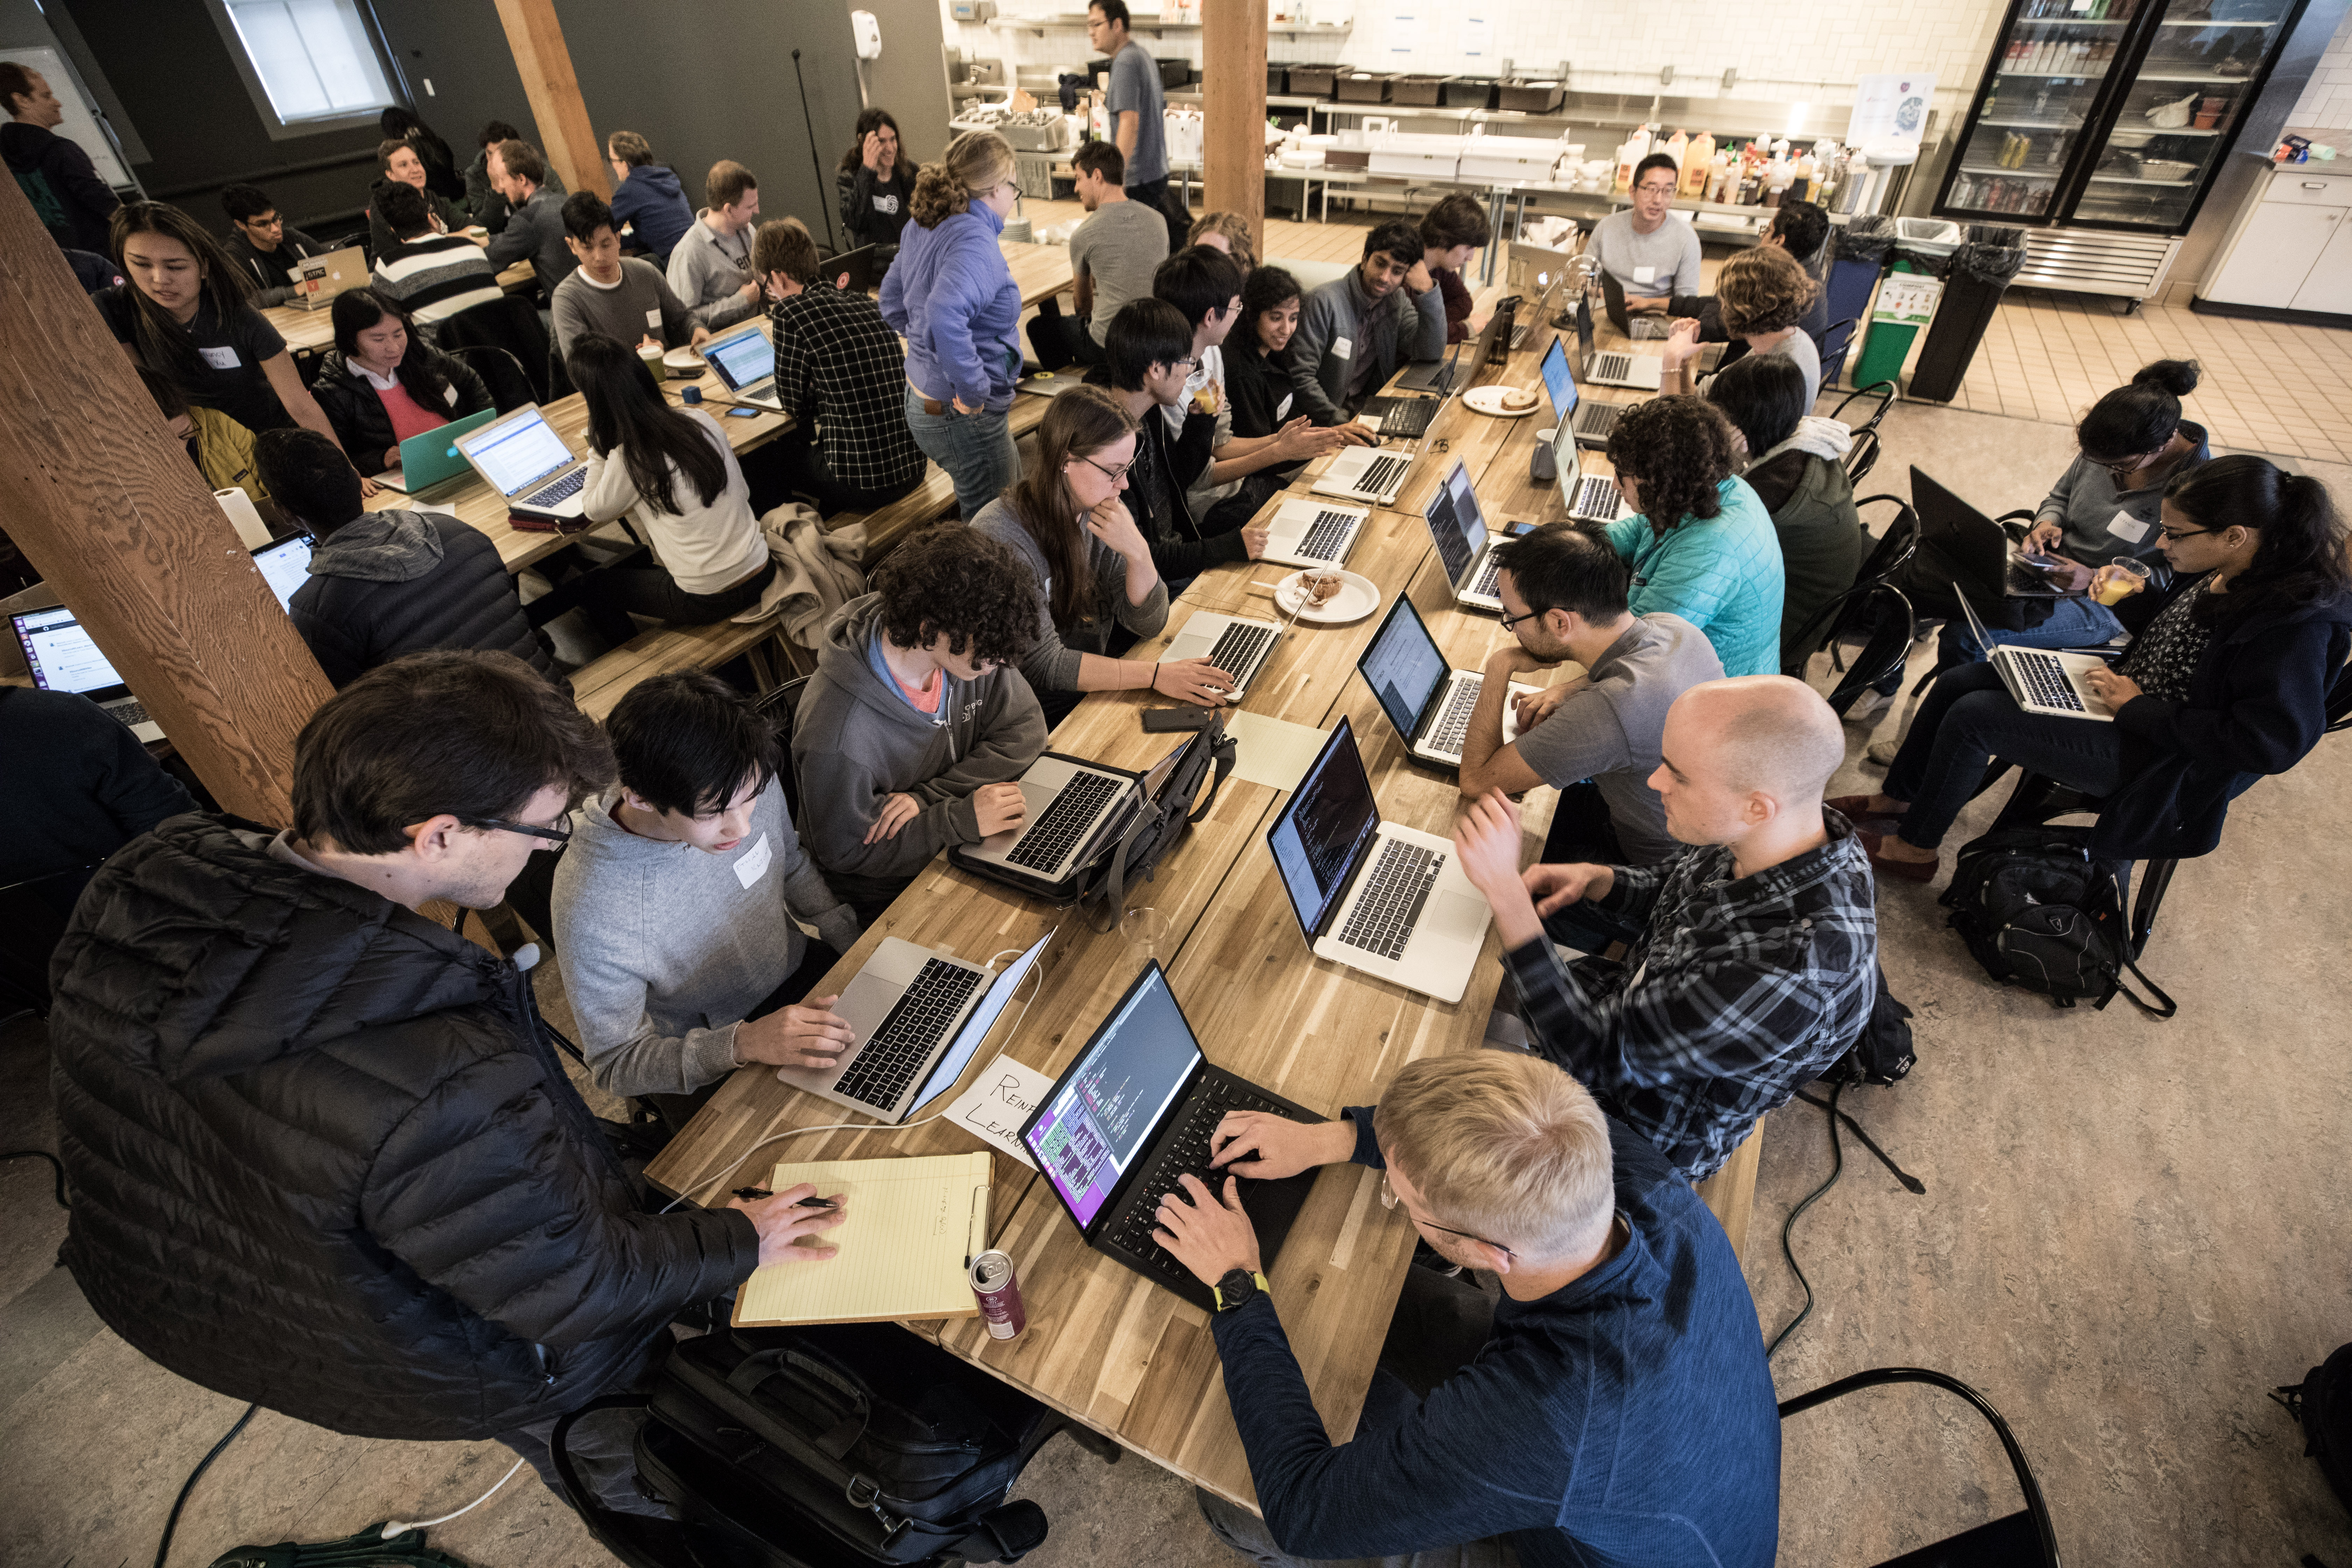
\includegraphics[height=3cm]{hackathon}
\end{figure}

\end{frame}